\documentclass[12pt]{article}
\usepackage[utf8]{inputenc}
\usepackage{amsmath}
\usepackage{tikz}
\usepackage{pgfplots}
\usepackage{array}
\pgfplotsset{compat=1.5}
\setlength\parindent{0pt}
\renewcommand{\arraystretch}{1.2}

\title{UGBS 618: Production and Operations Management\\
	Assignment 3}
\author{Oppey Geoff 10423631 \\
	Kelly Denning 10379353\\
	Akosua Krah Agyei	10637605\\
	Dennis Elorm Avuletey    10636922\\
	Adu Faustina	10391689\\}
\date{}

\begin{document}
	\maketitle
	
	a)\begin{align*}
		\text{Total Cost of Quality} &= \text{Cost of Quality Assurance} + \text{Cost of Not Conforming}. \\
		\text{Cost of Quality Assurance} &= \text{Prevention Cost} + \text{Appraisal Cost} \\
		\text{Cost of Not Conforming} &= \text{Internal Failure Cost} + \text{External Failure Cost}
	\end{align*} 
	
	The total cost of quality for each year from 2006 to 2010 have been computed and shown in the table below.
	
	\begin{table}[h]
		\begin{center}
			\begin{tabular}{l|ccccc}
				\hline
				&\multicolumn{5}{c}{Year}  \\ 
				\hline
				&2006 & 2007 & 2008 & 2009 & 2010 \\
				\hline
				Quality Costs\\
				Prevention & 3.2 & 10.7 & 28.3 & 42.6 & 50.0 \\
				Appraisal & 26.3 & 29.2 & 30.6 & 24.1 & 19.6 \\
				\hline
				Cost of Achieving Quality (A) & 2 9.5 & 39.9 & 58.9 & 66.7 & 69.6\\
				\hline
				Internal failure & 39.1 & 51.3 & 48.4 & 35.9 & 32.1 \\
				External failure & 118.6 & 110.5 & 105.2 & 91.3 & 65.2 \\
				\hline
				Cost of Poor Quality (B) & 157.7 & 161.8 & 153.6 & 127.2 & 97.3 \\
				\hline
				Total Cost of Quality (A + B) & 187.2 & 201.7 & 212.5 & 193.9 & 166.9\\
				\hline
				\hline
			\end{tabular}
			\caption{All figures in \$'000}
		\end{center}
	\end{table}

\begin{align*}
	\text{Total failure cost as a percentage of Total Quality Costs} &= \frac{\text{Total Cost of Not Conforming}}{\text{Total Cost of Quality}} * 100\%
\end{align*}

This has been computed for all years and shown in the table below.\\

\renewcommand{\arraystretch}{2.5}

	\begin{table}[h]
		\begin{center}
		\begin{tabular}{c|p{4in}}
			\hline
			Year & Failure cost as a percentage of Total Quality Cost  \\ \hline
			2006 & $\dfrac{157.7}{187.2} * 100 = 84.2415\% $  \\ \hline 
			2007 & $\dfrac{161.8}{201.7} * 100 = 80.2181$ \% \\ \hline
			2008 & $\dfrac{153.6}{212.5} * 100 = 72.2823$  \\ \hline
			2009 & $\dfrac{127.2}{193.9} * 100 = 65.6008\%$  \\ \hline
			2010 & $\dfrac{97.3}{166.9} * 100 = 58.2984\% $  \\ \hline
		\end{tabular}
		\caption{All percentages rounded to 4 d.p}
	\end{center}
	\end{table}


As shown in Table 2, the failure cost as a percentage of total cost has been declining steadily from 2006 to 2010. This has also been illustrated in the graph below.

\begin{center}
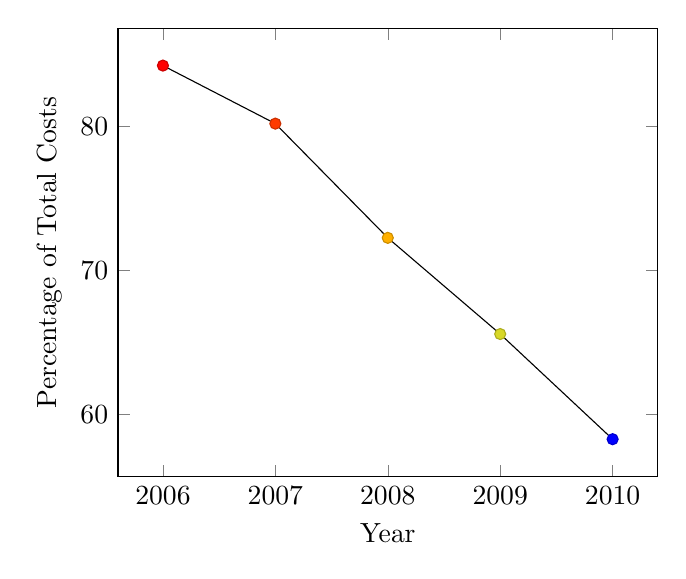
\begin{tikzpicture}
\begin{axis}[
		xlabel = Year,
		ylabel = Percentage of Total Costs,
		x tick label style={
			/pgf/number format/1000 sep=}
	]
	\addplot[
	scatter
	] table {
		x	y
		2006	84.24
		2007	80.21
		2008	72.28
		2009	65.60
		2010	58.30
	};
\end{axis}
\end{tikzpicture}
\end{center}

The decline could be attributed to the quality management program. It seems the company is spending more on prevention and appraisal, leading to lower failures, which has caused lesser internal and external failure costs.

\vspace{0.5cm}

b) 	\begin{align*}
			\text{Prevention cost as a percentage of Total Cost}\\ 
			&= \frac{\text{Prevention Cost}}{\text{Total Cost of Quality}} * 100\%\\
			\text{Appraisal cost as a percentage of Total cost}\\
			&= \frac{\text{Appraisal Cost}}{\text{Total Quality Cost}} * 100\%
	\end{align*}

Calculations for each year from 2006 to 2010 are shown in the table below.

	\begin{table}[h]
	\begin{center}
	\begin{tabular}{c|m{3in}|m{3in}}
		\hline
		Year & Prevention Cost as a Percentage of Total Quality Cost & Appraisal Cost as a Percentage of Total Quality Cost \\ 
		\hline
		2006 & $\dfrac{3.2}{187.2} * 100 = 1.71\% $ 
		& $\dfrac{26.3}{187.2} * 100 = 14.06\%$ \\ 
		\hline 
		2007 & $\dfrac{10.7}{201.7} * 100 = 5.30\%$ \% 
		& $\dfrac{29.2}{201.7} * 100 = 14.48\%$\\ 
		\hline
		2008 & $\dfrac{28.3}{212.5} * 100 = 13.32\%$  
		& $\dfrac{30.6}{212.5} * 100 = 14.40\%$\\  
		\hline
		2009 & $\dfrac{42.6}{193.9} * 100 = 21.97\%$  
		& $\dfrac{24.1}{193.9} * 100 = 12.43\%$\\ 
		\hline
		2010 & $\dfrac{50.0}{166.9} * 100 = 29.96\% $  
		& $\dfrac{19.6}{166.9} * 100 = 11.74\%$ \\ 
		\hline
	\end{tabular}
	\caption{All percentages rounded to 2 d.p}
	\end{center}
	\end{table}	

It appears that the company is investing more in prevention activities such as training staff, careful planning of the production process and ensuring that processes conform to quality specification whiles at the same time keeping its appraisal system of inspection and testing constant. This is done with the aim of keeping internal and external failure costs low.\\

c) The quality-sales and quality-cost indices may be computed using the formulas shown below.

	\begin{align*}
		\text{Quality Sales Index} &= \frac{\text{Total Cost of Quality}}{\text{Sales}} * 100\\
		\text{Quality Manufacturing Index} &= \frac{\text{Total Cost of Quality}}{\text{Manufacturing Cost}} * 100\\
	\end{align*}
	
	The indices are computed and shown in the table below.
	
	\begin{table}[h]
	\begin{center}
	\begin{tabular}{l|c|c}
		\hline
		Year & Quality Sales Index & Quality Manufacturing Cost Index \\ \hline
		2006 & $\dfrac{187.2}{2700.6} * 100 = 6.93$ 
		& $\dfrac{187.2}{420.9} * 100 = 44.48$ \\ \hline
		2007 & $\dfrac{201.7}{2690.1} * 100 = 7.50$ 
		& $\dfrac{201.7}{423.4} * 100 = 47.64$ \\ \hline
		2008 & $\dfrac{212.5}{2705.3} * 100 = 7.85$ 
		& $\dfrac{212.5}{424.7} * 100 = 50.04$ \\ \hline
		2009 & $\dfrac{193.9}{2310.2} * 100 = 8.39$ 
		& $\dfrac{193.9}{436.1} * 100 = 44.46$ \\ \hline
		2010 & $\dfrac{166.9}{2880.7} * 100 = 5.79$ 
		& $\dfrac{166.9}{435.5} * 100 = 38.32$ \\ \hline
	\end{tabular}
	\caption{All indices rounded to 2 d.p.}
	\label{}
	\end{center}
	\end{table}

From these indices, one cannot really tell whether the quality improvement programme was effective or not.

d) Prevention Costs include:
\begin{itemize}
	\item Process design cost: The costs involved in designing a new product or process.
	\item Training cost: Costs of improving workers' competence.
	\item Quality planning cost
	\item Quality engineering cost
	\item Equipment testing cost
\end{itemize}

Appraisal Costs include:
\begin{itemize}
	\item Quality audit cost
	\item Supplier rating cost
	\item Inspection and testing cost
\end{itemize}

Internal failure costs include
\begin{itemize}
	\item Scrap cost: Costs incurred when poor quality parkas are disposed off.
	\item Rework cost: Cost of mending torn parkas.
	\item Process downtime cost: The cost of time lost due to a breakdown of the production process. For example, the sewing machines break down and need to be repaired.
	\item Process failure cost
\end{itemize}

External failure costs include
\begin{itemize}
	\item Customer complaint cost: Costs incurred to receive and resolve complaints from customers.
	\item Verification cost: Costs involved in verifying customer warranty claims.
	\item Product return cost: Costs incurred to receive poor quality products and issue new ones to customers.
	\item Price down-grading cost: Loss in selling price due to lower prices offered in order to sell poor quality goods. 
	\item Lost sales cost: Costs to the company when it loses potential or existing customers through bad-mouthing of the company by other customers.
	\item Warranty cost: Resources lost when the company settles legitimate warranty claims.
\end{itemize}
\end{document}